\chapter{sheet-26 : Identical Particles}

%%% defining graphics path
\ifpdf
\graphicspath{{Chapter26/figs/}}
\else
\graphicspath{{Chapter26/figs/}}
\fi



%\setcounter{chapter}{26}


\begin{Large}
	\noindent
	{\bf Lecture 26 \newline
		Identical Particles}
\end{Large}
\vspace{1 cm}

\section{Indistinguishability of identical particles}
Two particles are said to be identical when they cannot be distinguished by means of any intrinsic property such as mass, electric
charge, spin etc. Thus all the electrons in the universe are identical, as are all the protons, all the hydrogen atoms. But,
an electron and a positron are not identical, since, although they have the same mass and same spin, they have different
electric charges.

\paragraph{}
In classical mechanics, identical particles can, in principle, be distinguished from one another by observing their individual paths or by 
other means like physically labeling them, by different colors, for example. In quantum mechanics the situation is entirely different. By
virtue of the uncertainty principle, the concept of the path of an electron (or any microscopic particle) ceases to have any
meaning. If the position of an electron is exactly known at a given instant, its coordinates have no definite values even at the
next instant. Hence by localizing and numbering the electrons at some instant, we make no progress towards identifying them at subsequent instants. If we localize one of the electrons at a subsequent instant at some at some point in space, we cannot say which of the electrons has been detected at this point.

\paragraph{}
Thus, in quantum mechanics, there is in principle no possibility of separately following each of a number of similar particles and thereby distinguishing them. We may say that, in quantum mechanics, identical particles entirely lose their ``individuality", i.e., they are
indistinguishable. The principle of indistingushability of similar particles, play a fundamental part in the quantum theory of systems composed of identical particles.  

\subsection{The wave function of two identical particles}
Let us start by considering a system of only two identical particles. Because of the identity of the particles, the states of the
system obtained from each other by interchanging the two particles must be completely equivalent physically. This means that, as a 
result of this interchange, the wave function of the system can change only by an unimportant phase factor. Let $\psi(\xi_1, \xi_2)$ be the wave function of the system, $\xi_1$ and $\xi_2$ conventionally denoting the three coordinates and the spin projection for each particle. The we must have
\be
\psi(\xi_1, \xi_2) = e^{i\alpha}\psi(\xi_2, \xi_1)\, ,
\ee
where $\alpha$ is some real constant. By repeating the interchange, we return to the original state while the function $\psi$ gets multiplied by $e^{2i\alpha}$. Hence it follows that $e^{2i\alpha}=1$, or, $e^{i\alpha}=\pm 1$. Thus
\be
\psi(\xi_1, \xi_2) = \pm \psi(\xi_2, \xi_1)\, .
\ee
We thus reach the result that there are only two possibilities: the wave function is either \textit{symmetrical} (i.e., it is unchanged when the particles are interchanged) or \textit{antisymmetrical} (i.e., changes sign when this interchange is made). It is obvious that the wave functions of all the states of a given system must have the same symmetry; otherwise the wave function of a state which was a superposition of states of different symmetry would be neither symmetrical nor antisymmetrical.

\paragraph{}
This result can be immediately generalized to systems consisting of 
any number of identical particles. For it is clear from the identity 
of the particles that, if any pair of them has the property of being 
described by, say, symmetrical wave functions, any other pair of such 
particles has the same property. Hence the wave function of identical 
particles must either be unchanged when any pair of particles are 
interchanged (and hence when the particles are permuted in any 
manner), or change sign when any pair are interchanged. In the first 
case we speak of a symmetrical wave function, and in the second case 
of an antisymmetrical one. 


\subsection{Spin Statistics Theorem}	
The property of being described by symmetrical or antisymmetrical 
wave functions depends on the nature of the particles. Particles 
described by antisymmetrical functions are said to obey Fermi-Dirac 
statistics (or to be fermions), while those which are described by 
symmetrical functions are said to obey Bose-Einstein statistics (or to be 
bosons)? 

\paragraph{}
According to the laws of relativistic 
quantum mechanics, the statistics obeyed by particles is uniquely 
related to their spin: particles with half-integral spin are fermions, 
and those with integral spin are bosons. 


\subsection{Statistics of Composite Particles}
The statistics of complex particles is determined by the 
number of elementary fermions entering into their composition. 
For, an interchange of two identical complex particles is equivalent to 
the simultaneous interchange of several pairs of identical elementary 
particles. The interchange of bosons does not change the wave function, 
while the interchange of fermions changes its sign. Hence complex 
particles containing an odd number of elementary fermions obey 
Fermi statistics, while those containing an even number obey Bose statistics. 
This result is, of course, in agreement with the above rule, since 
a complex particle has an integral or a half-integral spin according as 
the number of particles with half-integral spin entering into its 
composition is even or odd. 

\paragraph{}
Thus atomic nuclei of odd mass number (i.e. containing an odd 
number of neutrons and protons) obey Fermi statistics, and those of 
even atomic number obey Bose statistics. For atoms, which contain both 
nuclei and electrons, the statistics is evidently determined by the parity 
of the sum of the mass number and the atomic number, i.e., $(-1)^{(A+Z)}$.

\subsection{Operators for s system of identical particles}
To say that two particles are identical means that there are no interactions that can distinguish them. Thus
any operator corresponding to a physical observable of a collection of $N$ identical particles must treat all the
particles on the same footing. Therefore, the operator must be a symmetric function of the coordinates.

\paragraph{}
Thus, for example, the Hamiltonian $H(\xi_1, \xi_2, \cdots, \xi_N)$ must remain unchanged under the interchange of any two particles, 
and hence under any permutation of coordinates. One calls such an operator symmetric operator.

\paragraph{}
A system of $N$ identical particles starting out in a completely symmetric, or antisymmetric state, must always remain in such a state.
This is because any perturbation $V(\xi_1, \xi_2, \cdots, \xi_N)$ that can act to change the state of the system, must be a completely symmetric function of the coordinates of the $N$ particles and therefore commutes with the permutation operator, i.e.,
\[ [\hat{P}, \hat{V}]= 0 . \]
Therefore, if $\hat{P}|\psi\rangle = \pm |\psi\rangle$, then
\[ \hat{P}\hat{V}|\psi\rangle = \hat{V}(\hat{P}|\psi\rangle) = \pm \hat{V}|\psi\rangle, \]
so that $\hat{V}|\psi\rangle$ has the same symmetry as $|\psi\rangle$.



% Section 2
\section{States of Noninteracting Identical Particles}
Suppose we have $N$ noninteracting identical particles each in the same potential well $V(r)$. The Hamiltonian of a single particle,
say particle 1,  in the well is 
\be
\hat{H}_0 (1) = \frac{\hat{p}_1^2}{2m} + V(\xi_1)\, .\
\ee
Let us write the orthonormal energy eigenstates of this Hamiltonian as $\phi_1(\xi_1), \phi_2(\xi_1), \cdots $ with corresponding energies
$\epsilon_1, \epsilon_2, \cdots$. The Hamiltonian for the $N$ particles in the well is just the sum of the individual energy operators of the particles, i.e.,
\be
\hat{H}= \hat{H}_0(1) + \hat{H}_0(2) + \cdots + \hat{H}_0(N) .
\ee
It is easy to write down solutions of the Schr\"{o}dinger equation
\be
\hat{H}\psi(\xi_1, \xi_2, \cdots, \xi_N) = E \psi(\xi_1, \xi_2, \cdots, \xi_N)\, .
\label{eq:se}
\ee
For example, 
\be
\psi(\xi_1, \xi_2, \cdots, \xi_N)= \phi_{\alpha_1}(\xi_1)\phi_{\alpha_2}(\xi_2)\cdots \phi_{\alpha_N}(\xi_N)
\label{eq:sol1}
\ee
is a solution which corresponds to the first particle in state $\alpha_1$ with energy $\epsilon_1$, the second particle in state
$\alpha_2$ with energy $\epsilon_2$, etc. The total energy of the system is simply
\be
E = \epsilon_{\alpha_1} + \epsilon_{\alpha_2}+ \cdots + \epsilon_{\alpha_N}\, .
\ee

\paragraph{}
In general, Eq. (\ref{eq:sol1}) is not an admissible solution for $N$ identical particles since it lacks the symmetry under interchange of any two particles. There are many other solutions to Eq. (\ref{eq:se}). Any permutations of $\xi_1, \xi_2, \cdots , \xi_n$ on the right hand side of Eq. (\ref{eq:sol1}) yields, in general, another solution to Eq. (\ref{eq:se}) with the same energy for the system of N identical particles.


\paragraph{}
To construct admissible eigenstates for $N$ identical particles, we must take linear combination of states of the form Eq. (\ref{eq:sol1}) that is completely symmetric for bosons or completely antisymmetric for fermions.

\subsection{Identical Fermions}
For two identical fermions, the antisymmetric state is
\be
\psi_a(1,2)=\frac{1}{\sqrt{2}}\, \left[ \phi_{\alpha_1}(1)\phi_{\alpha_2}(2)- \phi_{\alpha_1}(2)\phi_{\alpha_2}(1)\right]
\ee
and, generally for $N$ particles 
\be
\psi_a(1,2,\cdots, N)= \frac{1}{\sqrt{N!}}\, \sum_p (-1)^P P \phi_{\alpha_1}(1)\phi_{\alpha_2}(2)\cdots \phi_{\alpha_1}(N)
\label{eq:perm}
\ee
where the sum is over all the $N!$ permutations of the arguments $1,2,\cdots, N$ of the single particle wave functions. These arguments represent the space and the spin coordinates $\xi_1,\xi_2,\cdots,\xi_N$ of the fermions.  If the permutation is even, i.e., if the permutation 
can be obtained by an even number of interchanges of pairs of particles (i.e., even number of transpositions), then there is a plus sign.
If the permutation is odd, there is a minus sign.  Eq. (\ref{eq:perm}) can be written in the determinant form
\be
\psi_a(1,2,\cdots, N)= \frac{1}{\sqrt{N!}}\,
\begin{vmatrix}
	\phi_{\alpha_1}(1) & \phi_{\alpha_1}(2) & \cdots & \phi_{\alpha_1}(N) \\
	\phi_{\alpha_2}(1) & \phi_{\alpha_2}(2) & \cdots & \phi_{\alpha_2}(N) \\
	\vdots & \vdots & & \vdots \\
	\phi_{\alpha_N}(1) & \phi_{\alpha_N}(2) & \cdots & \phi_{\alpha_N}(N) 
\end{vmatrix}\, .
\label{eq:slater}
\ee
These determinants of one-particle states are called Slater determinants. The antisymmetry of Eq. (\ref{eq:slater}) is immediately
apparent since interchange of any two columns introduces a factor of $-1$. The normalization is $1/\sqrt{N!}$ since Eq. (\ref{eq:slater})
consists of $N!$ mutually orthogonal terms.

\paragraph{}
From the Slater determinant it is also apparent that if two or more sets of individual states are identical, i.e., 
$\alpha_i=\alpha_j$ etc., the wave function (\ref{eq:slater}) vanishes. As a result only one fermion can occupy a given individual quantum state. This statement is known as {\bf Pauli exclusion principle}.



\subsection{Identical Bosons}
Let $\alpha_1, \alpha_2, \cdots , \alpha_N$ be the quantum numbers of the single particle states occupied by $N$ identical non-interacting bosons. Some of the quantum numbers may be the same.
For a system of bosons, the wave function $\psi(1,2,\cdots,N)$ is given by a 
sum of products of the form 
\be
\phi_{\alpha_1}(1)\phi_{\alpha_2}(2)\cdots \phi_{\alpha_N}(N)
\ee
with all possible permutations of the indices $(1,2,\cdots,N)$. 
This sum clearly possesses the required symmetry property. Thus, for 
example, for a system of two particles in different states $(\alpha_1 \neq \alpha_2)$
\be 
\psi(1,2) = \frac{1}{\sqrt{2}}\, \left[ \phi_{\alpha_1}(1)\phi_{\alpha_2}(2) + \phi_{\alpha_1}(2)\phi_{\alpha_2}(1)\right]\, .
\ee
The factor $1/\sqrt{2}$ is introduced for normalization purposes; all the 
functions $\phi_1,\phi_2, \cdots$ are orthogonal and are supposed normalized. 
In the general case of a system containing an arbitrary number $N$ of 
particles, the normalized wave function is 
\be
\psi= \left( \frac{N_1!N_2!\ldots }{N!}\right)^{1/2}\sum P \phi_{\alpha_1}(1)\phi_{\alpha_2}(2)\cdots \phi_{\alpha_N}(N)\, ,
\label{eq:boson}
\ee
where the sum is taken over all distinct permutations of the particles. 
The numbers $N_i$ represent how many of the suffixes 
have the same value $\alpha_i$, i.e., how many identical bosons are accommodated in the same single particle state $\phi_{\alpha_i}$.
Obviously,  $\sum N_i = N$. In the integration of $|\psi|^2$ over the space and spin coordinates  
$\xi_1,\xi_2, \cdots , \xi_N$, all terms vanish except the squared modulus of each 
term. Since the total number of terms in the sum (\ref{eq:boson}) is evidently 
\[ \frac{N!}{N_1!N_2! \ldots}, \]
the normalization factor in (\ref{eq:boson}) is obtained.


\subsubsection{Example}
Griffiths page 217

Suppose we have two noninteracting particles, both of mass $m$ in an infinite square well. The one-particles states are:
\[ \psi_n(x)=\sqrt{\frac{2}{a}}\, \sin \left(\frac{n\pi}{a}x \right), \quad E_n = n^2 K \]
where $K=\pi^2\hbar^2/2ma^2$. If the particles are distinguishable, with particle 1 in state $n_1$ and particle 2 in state $n_2$, the composite wave function is the simple product
\[ \psi_{n_1n_2}(x_1,x_2) = \psi_{n_1}(x_1) \psi_{n_2}(x_2), \quad E_{n_1n_2}=(n_1^2+n_2^2)K. \]
For example, the ground state is
\[ \psi_{11}= \frac{2}{a} \sin (\pi x_1/a)\sin(\pi x_2/a), \quad E_{11}= 2K; \]
the first excited state is doubly degenerate
\[ \psi_{12}=  \frac{2}{a} \sin (\pi x_1/a)\sin(2\pi x_2/a), \quad E_{12}= 5K, \]
\[ \psi_{21}= \frac{2}{a} \sin (2\pi x_1/a)\sin(\pi x_2/a), \quad E_{21}= 5K; \]
and so on. 

\paragraph{}
If the two particles are identical bosons, the ground state is unchanged, but the first excited state is nondegenerate:
\[ \frac{\sqrt{2}}{a}\, \left[ \sin (\pi x_1/a)\sin(2\pi x_2/a) + \sin (2\pi x_1/a)\sin(\pi x_2/a)\right] \]
still with energy $5K$. 

\paragraph{}
And, if the particles are identical fermions, there is no state with energy $2K$; the ground state is
\[ \frac{\sqrt{2}}{a}\, \left[ \sin (\pi x_1/a)\sin(2\pi x_2/a) - \sin (2\pi x_1/a)\sin(\pi x_2/a)\right],\]
and its energy is $5K$.



\subsection{Exchange Forces}
From Griffiths

Consider a state consisting of two non interacting particles. Suppose one particle is in the state $\psi_a$ and the other in the state $\psi_b$. The two states are orthogonal and normalized. If the two particles are distinguishable, and particle number 1 is in the state $\psi_a$, then the combined wave function is
\be
\psi(x_1,x_2) = \psi_a(x_1)\psi_b(x_2).
\label{eq:dis}
\ee
If they are identical bosons, the composite wave function is 
\be
\psi_+(x_1,x_2) = \frac{1}{\sqrt{2}}\, \left[ \psi_a(x_1)\psi_b(x_2) + \psi_b(x_1)\psi_a(x_2) \right];
\label{eq:bose1}
\ee
and if they are identical fermions, the wave function is
\be
\psi_-(x_1,x_2) = \frac{1}{\sqrt{2}}\, \left[ \psi_a(x_1)\psi_b(x_2) - \psi_b(x_1)\psi_a(x_2) \right].
\label{eq:fermi1}
\ee
Let us calculate the expectation value of the square of the separation distance between the two particles:
\be
\langle(x_1-x_2)^2\rangle = \langle x_1^2 \rangle + \langle x_2^2 \rangle - 2 \langle x_1 x_2 \rangle\, .
\label{eq:sep}
\ee

\subsubsection{Case 1: Distinguishable Particles.}
For the wave function in Equation (\ref{eq:dis}), we have
\[
\langle x_1^2 \rangle = \int x_1^2 |\psi_a(x_1)|^2dx_1\, \int |\psi_b(x_2)|^2dx_2 = \langle x^2 \rangle_a
\]
i.e., the expectation value of $x^2$ in the one-particle state $\psi_a$. We also have
\[
\langle x_2^2 \rangle = \int  |\psi_a(x_1)|^2dx_1\, \int x_2^2 |\psi_b(x_2)|^2dx_2 = \langle x^2 \rangle_b\, ,
\]
and
\[
\langle x_1 x_2 \rangle = \int x_1 |\psi_a(x_1)|^2dx_1\, \int x_2 |\psi_b(x_2)|^2 dx_2 = \langle x \rangle_a \langle x \rangle_a\, .
\]
In this case, then
\be
\langle(x_1-x_2)^2\rangle_d = \langle x^2 \rangle_a + \langle x^2 \rangle_b - 2 \langle x \rangle_a \langle x \rangle_b \,.
\label{eq:sepd}
\ee
Incidentally, the answer would, of course, be the same if particle 1 had been in state $\psi_b$, and particle 2 in state $\psi_a$.


\subsubsection{Case 2: Identical Particles}
For the wave functions in Equations (\ref{eq:bose1}) and (\ref{eq:fermi1}),
\begin{eqnarray*}
	\langle x_1^2 \rangle & = & \frac{1}{2}\, \left [ \int x_1^2 |\psi_a(x_1)|^2 dx_1 \int |\psi_b(x_2)|^2 dx_2 \right . \\
	& & + \int x_1^2 |\psi_b(x_1)|^2 dx_1 \int |\psi_a(x_2)|^2 dx_2 \\
	& &  \pm \int x_1^2 \psi_a(x_1)^* \psi_b(x_1)dx_1 \int \psi_b(x_2)^* \psi_a(x_2) dx_2 \\
	& & \left .\pm \int x_1^2 \psi_b(x_1)^* \psi_a(x_1)dx_1 \int \psi_a(x_2)^* \psi_b(x_2) dx_2 \right ] \\
	& = & \frac{1}{2}\, \left [ \langle x^2 \rangle_a + \langle x^2 \rangle_b \pm 0 \pm 0 \right ] = \frac{1}{2}\, \left(
	\langle x^2 \rangle_a + \langle x^2 \rangle_b \right ).  
\end{eqnarray*}
Similarly,
\[
\langle x_2^2 \rangle = \frac{1}{2} \left ( \langle x^2 \rangle_b + \langle x^2 \rangle_a \right).
\]
(Naturally, $ \langle x_1^2 \rangle= \langle x_2^2 \rangle$, since one cannot tell them apart). But
\begin{eqnarray*}
	\langle x_1x_2 \rangle & = & \frac{1}{2}\, \left[ \int x_1|\psi_a(x_1)|^2dx_1 \int x_2|\psi_b(x_2)|^2dx_2 \right . \\
	& & + \int x_1|\psi_b(x_1)|^2dx_1 \int x_2|\psi_a(x_2)|^2dx_2 \\
	& & \pm \int x_1 \psi_a(x_1)^* \psi_b(x_1) dx_1 \int x_2 \psi_b(x_2)^* \psi_a(x_2)dx_2 \\
	& & \left . \pm \int x_1 \psi_b(x_1)^* \psi_a(x_1) dx_1 \int x_2 \psi_a(x_2)^* \psi_b(x_2)dx_2 \right ] \\
	& = & \frac{1}{2} \, \left[ \langle x \rangle_a \langle x \rangle_b + \langle x \rangle_b \langle x \rangle_a 
	\pm \langle x \rangle_{ab} \langle x \rangle_{ba} \pm \langle x \rangle_{ba}\langle x \rangle_{ab} \right ] \\
	& = & \langle x \rangle_a \langle x \rangle_b \pm | \langle x \rangle_{ab}|^2 \, , 
\end{eqnarray*}
where
\be
\langle x \rangle_{ab} = \int x \psi_a(x)^*\psi_b(x) dx\, .
\label{eq:xab}
\ee
Evidently
\be
\langle (x_1-x_2)^2 \rangle_{\pm} = \langle x^2 \rangle_a + \langle x^2 \rangle_b - 2\langle x \rangle_a \langle x \rangle_b
\mp 2|\langle x \rangle_{ab}|^2\, .
\label{eq:sepi}
\ee

\paragraph{}
Comparing Eqs. (\ref{eq:sepd}) and (\ref{eq:sepi}), we see that the difference lies in the final term:
\be
\langle (\Delta x)^2 \rangle_{\pm} = \langle (\Delta x)^2 \rangle_d \mp 2|\langle x \rangle_{ab}|^2.
\ee
Identical bosons (the upper signs) tend to be somewhat closer together, and identical fermions (the lower signs) somewhat further apart, than distinguishable particles in the same two states.		 Notice that $\langle x \rangle_{ab}$ \textit{vanishes} unless the two wave functions actually overlap [ if $\psi_a(x)$ is zero wherever $\psi_b(x)$ is nonzero, the integral in 
Eq. (\ref{eq:xab})	is itself zero]. So, if $\psi_a$ represents an electron in an atom in Chicago and $\psi_b$ represents an
electron in an atom in Seattle, it's is not going to make a difference if you antisymmetrize the wave function or not. As 
a practical matter, therefore it's okay to pretend that electrons with nonoverlapping wave functions are distinguishable.

\paragraph{}
The interesting case is when there is some overlap of the wave functions. The system behaves as though there were a ``force
of attraction" between identical bosons pulling them closer together, and a ``force of repulsion" between identical fermions pushing them apart. We call it an {\bf exchange force}, although it is not really a force at all --- no physical agency is pushing on the particles; rather, it is purely a geometrical consequence of the symmetrization requirement. It is also a strictly quantum mechanical phenomenon, with no classical counterpart. Nevertheless, it has profound consequences. 

\paragraph{}
Consider, for example, the hydrogen molecule (H$_2$). Roughly speaking, the ground state consists of one electron in the atomic ground state centered on nucleus 1, and one electron in the atomic ground state centered at nucleus 2. If electrons were 
\textit{bosons}, the symmetrization requirement (or, if you like the ``exchange force") would tend to concentrate the electrons toward the middle between the two protons (Figure (\ref{fig:h2} a), and the resulting accumulation of negative charge would attract the protons inward, accounting for the {\bf covalent bond} that holds the molecule together. 
Unfortunately, electrons aren't bosons, they are fermions, and this means that the concentration of negative charge should
actually be shifted to the wings (Figure \ref{fig:h2} b), tearing the molecule apart.
\begin{figure}[!ht]
	\centering
	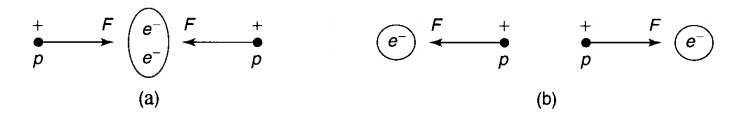
\includegraphics[width=\linewidth]{h2molecule.jpg}
	\caption{Schematic picture of the covalent bond: (a) symmetric configuration produces attractive force; (b) antisymmetric configuration produces repulsive force.}
	\label{fig:h2}
\end{figure}

\paragraph{}
But, wait. We have been ignoring \textit{spin}. The complete state of an electron includes not only its position wave function, but also a spinor, describing the orientation of its spin\footnote{In the absence of coupling between spin and position, we are free to assume that the state is separable in its spin and spatial coordinates. This just says that the probability of getting spin up is independent of the location of the particle. In the presence of coupling, the general state of a particle is a linear combination
	$\psi_+(\vec{r}\,)\chi_+ + \psi_-(\vec{r}\,)\chi_-$.}:
\be
\psi(\vec{r}\,)\chi(s).
\ee
When we put together the two-electron state, it is the \textit{whole works}, not just the spatial part, that has to be antisymmetric with respect to exchange. Now, for a two-particle system where each particle has spin quantum number $s=1/2$, the singlet combination is antisymmetric (and hence would have to be joined with a \textit{symmetric} spatial function), whereas the three 
triplet states are all symmetric (and would require an \textit{antisymmetric} spatial function). Evidently, then, the singlet state should lead to bonding, and triplet to antibonding. Sure enough, the chemists tell us that covalent bonding requires the two electrons to occupy the singlet state, with total spin zero.\footnote{In casual language, it is often said that in the singlet state the two electrons are ``oppositely aligned" (one with spin up and the other with spin down). This is something of an over simplification, since the same could be said for the $m=0$ triplet state. The precise statement is that they are in the singlet configuration.}



% New Section
\section{The Helium Atom}
The basic Hamiltonian of the helium atom is give by
\be
\hat{H} = -\frac{\hbar^2}{2m}\, \nabla_1^2 -\frac{\hbar^2}{2m}\, \nabla_2^2 -\frac{1}{4\pi \epsilon_0}\, \frac{2e^2}{r_1} 
-\frac{1}{4\pi \epsilon_0}\, \frac{2e^2}{r_2} + \frac{1}{4\pi \epsilon_0}\, \frac{e^2}{r_{12}}\, .
\ee
Suppose the $e^2/4\pi\epsilon_0 r_{12}$ term were absent. Then, with the identity of the electron ignored, the wave function would be just the product of two hydrogenic wave functions with $Z=1$ changed to $Z=2$. The total spin is a constant of motion, so that the spin state is either a singlet (antisymmetric) or a triplet (symmetric). The spin states are
\begin{eqnarray}
^1\chi_0 & = & \frac{1}{\sqrt{2}}\, \left[ \alpha(1)\beta(2)-\alpha(2)\beta(1)\right ] \quad {\rm (antisymmetric)} \\
^3\chi_1 & = & \alpha(1)\alpha(2) \quad {\rm (symmetric)}\\
^3\chi_0 & = & \frac{1}{\sqrt{2}}\, \left[ \alpha(1)\beta(2) + \alpha(2)\beta(1) \right ] \quad {\rm (symmetric)} \\
^3\chi_{-1} & = & \beta(1)\beta(2) \quad {\rm (symmetric)}.
\end{eqnarray}

\paragraph{}
Suppose that one of the electrons is in the ground state $(nlm)=(100)$, and the other in an excited state $(nlm)$ with $n\neq 1$.
Then the spatial wave function of the two electrons would be
\be
\phi(\vec{r}_1,\, \vec{r}_2\,) = \frac{1}{\sqrt{2}}\, \left[ \phi_{100}(\vec{r}_1\,)\phi_{nlm}(\vec{r}_2\,)
\pm \phi_{100}(\vec{r}_2\,)\phi_{nlm}(\vec{r}_1\,) \right]
\ee
where the upper sign is for the spin-singlet state  and the lower sign is for the spin-triplet states. 


\subsubsection{Ground State}
First, we consider the ground state. In this case both the electrons are in the orbital state $n=1,l=0,m=0$, i.e., the orbital configuration is $(1s)^2$. In this configuration the space part of the wave function of the two-electron system must necessarily
be symmetric. Therefore, the spin state of the system must be the antisymmetric singlet so that the overall wave function which is the product of the spatial wave function and the spin wave function is antisymmetric. So we have
\begin{eqnarray}
\psi(\vec{r}_2,\, \vec{r}_2\,) & = & \psi_{100}(\vec{r}_1\,)\psi_{100}(\vec{r}_2\,)\; ^1\chi_0 \nonumber \\
& = & \frac{Z^3}{\pi a_0^3}\, e^{-Z(r_1+r_2)/a_0}\,\, ^1\chi_0 \;\;\; (Z=2)\, .
\end{eqnarray}
This unperturbed wave function gives
\[ E= 2 \times 4\left(- \frac{e^2}{(4\pi\epsilon_0)2a_0}\right) = -8E_{\rm{Ry}} = -8 \times 13.6\; {\rm eV} = -109\; {\rm eV}.\]
for the ground state energy, which is about 30\% larger in magnitude than the experimental value of $-78.8$ eV.

\paragraph{}
Next, in order to obtain a better value for the ground state energy we take into account the effect of the perturbing potential
$e^2/4\pi\epsilon_0 r_{12}$ in the Hamiltonian. In the first-order perturbation theory, 
\begin{eqnarray}
\Delta E = E^{(1)} & = & \langle 1s^2|e^2/4\pi\epsilon_0 r_{12}|1s^2\rangle \; (^1\chi_0^{\dagger}\, ^1\chi_0) \nonumber \\
& = & \int \psi_{100}^*(\vec{r}_1\,)\psi_{100}^*(\vec{r}_2\,) \frac{e^2}{4\pi\epsilon_0 r_{12}}
\psi_{100}(\vec{r}_1\,)\psi_{100}(\vec{r}_2\,) d^3r_1 d^3r_2 \nonumber \\
& = & \frac{Z^6}{\pi^2 a_0^6}\int e^{-2Z(r_1+r_2)/a_0} \frac{e^2}{4\pi\epsilon_0 r_{12}}d^3r_1 d^3r_2 \;\; (Z=2)\nonumber \\
& = & \left( \frac{5}{2}\right)\left(\frac{e^2}{4\pi\epsilon_0 2a_0} \right) = \left( \frac{5}{2} \right) E_{\rm Ry}.
\end{eqnarray}
After adding this energy shift, we have
\[
E_{(1s)^2} = (-8+5/2)E_{Ry} = -74.8 \; {\rm eV}\, , \]
which is very close to the experimental value
\[ E_{\rm exp} = -78.8 \; {\rm eV}. \]



\subsubsection{Excited State}
Let us briefly consider the excited states. We consider only the case in which one of the electrons is in the single particle ground state $(100)$, i.e., the 1s state, and the other electron in the excited state $(nlm)$ with $n \neq 1$. We write the energy of the state as
\[
E = E_{100} + E_{nlm} + \Delta E \]
where
\[
E_{100}= E_{1s} = - Z^2 \frac{e^2}{4\pi \epsilon_0 2 a_0} \]
and for hydrogenic atoms
\[ E_{nlm} = E_{n} = - Z^2 \left (\frac{e^2}{4\pi \epsilon_0 2 a_0}\right) \, \frac{1}{n^2}\, . \]
The energy correction $\Delta E$ is
\be
\Delta E = \int \psi^*(\chi; \vec{r}_1\, \vec{r}_2\,) \frac{e^2}{4\pi\epsilon_0 r_{12}}\, \psi(\chi; \vec{r}_1\, \vec{r}_2\,)
\ee
where $\chi$ represents the spin state of the two electrons. We have
\[ \psi(\chi; \vec{r}_1\, \vec{r}_2\,) = \psi(\vec{r}_1\, \vec{r}_2\,) \chi \]
and
\[ \psi^*(\chi; \vec{r}_1\, \vec{r}_2\,) = \chi ^{\dagger} \psi^*( \vec{r}_1\, \vec{r}_2\,)\, . \]
Since the operator $e^2/4\pi\epsilon_0 r_{12}$ does not involve spin, it is clear that singlet and triplet states are separated and that the three triplet spin states remain degenerate.

\paragraph{}
For the singlet (triplet) states we have
\be
\begin{split}
	\Delta E_{\rm \begin{array}{l}{\rm singlet}\\{\rm triplet}\end{array} } = \int \frac{1}{\sqrt{2}}\, \left[ 
	\psi_{100}(\vec{r}_1\,)\psi_{nlm}(\vec{r}_2\,) \pm \psi_{100}(\vec{r}_2\,)\psi_{nlm}(\vec{r}_1\,)\right]^* 
	\frac{e^2}{4\pi\epsilon_0 r_{12}} \\
	\times \frac{1}{\sqrt{2}}\, \left[ 
	\psi_{100}(\vec{r}_1\,)\psi_{nlm}(\vec{r}_2\,) \pm \psi_{100}(\vec{r}_2\,)\psi_{nlm}(\vec{r}_1\,)\right]d^3r_1 d^3r_2
\end{split}
\ee
We can write the above equation as
\be
\Delta E_{\rm \begin{array}{l}{\rm singlet}\\{\rm triplet}\end{array} } = I \pm J
\ee
where
\be
I = \int d^3r_1\int d^3r_2 \, |\psi_{100}(\vec{r}_1\,)|^2\,  |\psi_{nlm}(\vec{r}_2\,)|^2 \frac{e^2}{4\pi\epsilon_0 r_{12}} 
\ee
and
\be
J = \int d^3r_1\int d^3r_2 \, \psi_{100}^*(\vec{r}_1\,)\psi_{nlm}^*(\vec{r}_2\,)\, \frac{e^2}{4\pi\epsilon_0 r_{12}}\,
\psi_{100}(\vec{r}_2\,)\psi_{nlm}(\vec{r}_1\,)
\ee
The upper (lower) sign goes with spin singlet (triplet) states. Obviously, $I$ is positive. We can show that $J$ is also positive. So the net result is such that for the same configuration $(100)^1(nlm)^1$, the spin singlet state lies higher, as shown in the figure below.
\begin{figure}[!ht]
	\centering
	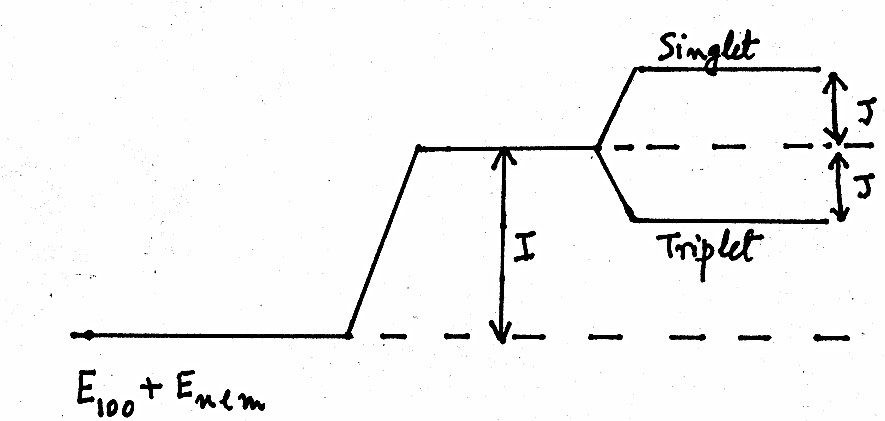
\includegraphics[width=\linewidth]{singlettriplet.jpg}
	\caption{ Removal of degeneracy between the singlet and triplet states of helium atom in the first order perturbation. }
	\label{fig:singlettriplet}
\end{figure}

\noindent
The physical interpretation for this is as follows:
\noindent
In the singlet case, the space function is symmetric and the electrons have a tendency to come close to each other. Therefore,
the electrostatic repulsion between the electrons is more serious; hence a higher energy results. In the triplet case, the space function is antisymmetric and the electrons tend to avoid each other.

\paragraph{}
Helium in spin-singlet state is known as parahelium, while helium in the spin-triplet state is known as orthohelium. Each configuration of the two electrons (except for the ground state configuration) splits into the para state and the ortho state, the para state lying higher in energy. For the ground state, only parahelium is possible. The figure below is a schematic energy level diagram for the low-lying configurations of the helium atom.

\begin{figure}[!ht]
	\centering
	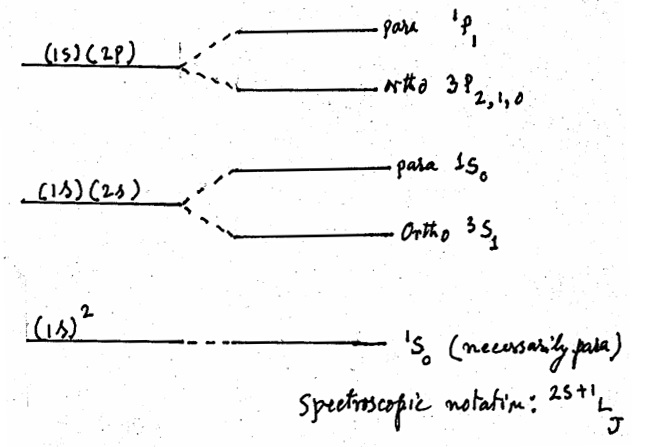
\includegraphics[width=\linewidth]{energylevel.jpg}
	\caption{ Energy levels for the low-lying configurations of the helium atom. The energy levels on the left
		of the diagram shows the mean of the ortho and para states, i.e., what the energy levels would have been in a given configuration if the electrons were distinguishable particles.}
	\label{fig:energylevel}
\end{figure}

\newpage
\section{Collision Between Identical Particles}
Read Bransden and Joachain, page 620.

Collisions between identical particles are particularly interesting as a direct illustration 
of the fundamental differences between classical and quantum mechanics. We shall 
examine first the elastic scattering of two identical spinless bosons and then analyze 
elastic collisions between two identical spin-1/2 fermions. 

\subsection{Scattering of Two Identical Spinless Bosons}
Let us consider the elastic scattering of two identical bosons of mass m. For simplicity 
we shall consider only the case of spinless bosons. We work in the centre-of-mass 
system, in which the time-independent Schrodinger equation is 
\be
\left[ -\frac{\hbar^2}{2 \mu} + V(r) \right] \psi(\vec{r}\,) = E \psi(\vec{r}\,) 
\ee
where $\mu =m/2$ is the reduced mass and $\vec{r} = \vec{r}_1 - \vec{r}_2$ is the relative position vector of 
the two colliding particles. The situation in the center-of-mass system is illustrated in 
Fig. (\ref{fig:collision1}). 
\begin{figure}[!ht]
	\centering
	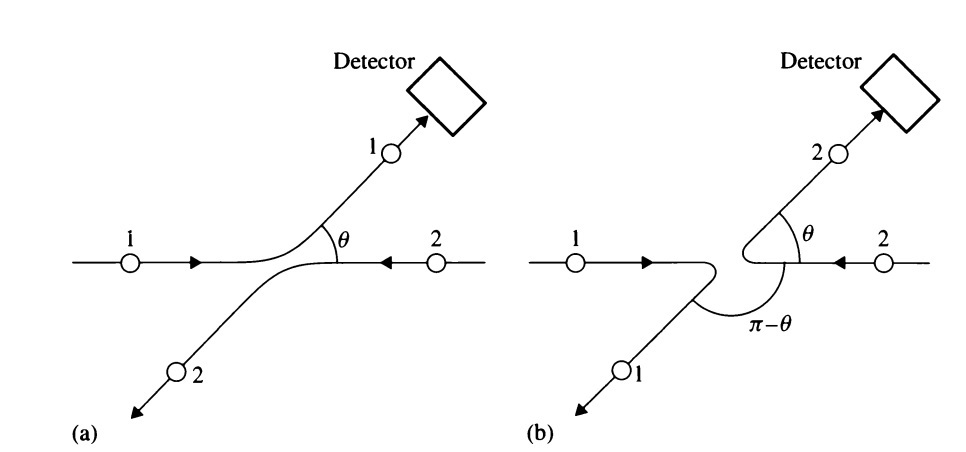
\includegraphics[width=\linewidth]{collision1.jpg}
	\caption{ The scattering of Identical particles in the centre-of-mass frame.}
	\label{fig:collision1}
\end{figure}


Two identical particles 1 and 2 approach one another, moving parallel to 
the z-axis in opposite directions. After an elastic collision the velocity of each particle 
is changed in direction but remains unchanged in magnitude. A detector counts the 
particles scattered into the direction characterized by the polar angles $(\theta,\phi)$. Since the 
particles 1 and 2 are identical, there is no way of deciding whether a particle recorded 
by the detector results from a collision event in which particle 1 is scattered in the 
direction $(\theta, \phi)$ (see Fig. \ref{fig:collision1} (a)), or from a collision process in which particle 2 
is scattered in that direction, so that particle 1 is scattered in the opposite direction 
$(\pi-\theta, \phi+\pi)$ (see Fig. \ref{fig:collision1} (b)). 

\paragraph{}
In classical mechanics the differential cross-section for scattering in the direction 
$(\theta,\phi)$ would simply be the sum of the differential cross-sections for observation of 
particle 1 and particle 2 in that direction. If the same were to be true in quantum 
mechanics, we would obtain for the differential cross-section the `classical' result 
\be
\frac{d\sigma_{cl}}{d\Omega} = \left| f(\theta, \phi)\right|^2 + \left| f(\pi-\theta, \phi + \pi)\right|^2
\label{eq:dcs1}
\ee
where $f(\theta, \phi)$ is the center-of-mass amplitude for scattering in the direction $(\theta, \phi)$.
The amplitude $f(\theta,\phi)$ is related to the asymptotic behavior of the wave function $\psi(\vec{r}\,)$ satisfying the usual boundary condition
\be
\psi(\vec{r}\,) \sim_{r\rightarrow \infty} e^{ikz} + f(\theta, \phi)\, \frac{e^{ikr}}{r} \, . 
\label{eq:bc}
\ee
However, we shall now show that the expression (\ref{eq:dcs1}) is incorrect.

\paragraph{}
Indeed, we have seen that wave functions 
describing systems of identical particles must be properly symmetrized with respect to 
permutations of the particles. In particular, a wave function describing a system 
of identical bosons must be completely symmetric. Thus, in the case of two identical 
spinless bosons, the wave function must be symmetric under the interchange of the 
spatial coordinates of the two particles. Now the interchange $\vec{r}_1 \leftrightarrow \vec{r}_2$ corresponds to 
replacing the relative position vector $\vec{r}$ by $-\vec{r}$, which in polar coordinates corresponds 
to $(r, \theta, \phi)$ being replaced by $(r, \pi-\theta, \phi+\pi)$. The wave function $\psi(\vec{r}\,)$ satisfying the 
boundary condition (\ref{eq:bc}) does not have the required symmetry, but the symmetric 
combination 
\[ \psi_+(\vec{r}\,) = \psi(\vec{r}\,) + \psi(-\vec{r}\,) \]
is also a solution of the Schr\"{o}dinger equation and does have the required symmetry, i.e., 
$\psi_+(-\vec{r}\,) = \psi_+(\vec{r}\,)$. Using Eq. (\ref{eq:bc}), the asymptotic form of $\psi_+(\vec{r}\,)$ is
\be
\psi_+(\vec{r}\,) \sim_{r\rightarrow \infty} \left[ e^{ikz}+e^{-ikz}\right] +
\left[ f(\theta, \phi)+f(\pi-\theta, \phi+\pi)\right]\,\frac{e^{ikr}}{r} \, .
\ee
The amplitude of the spherically outgoing wave is the symmetric amplitude
\be
f_+(\theta,\phi)=f(\theta,\phi)+f(\pi-\theta,\phi+\pi) \, ,
\ee
so that the differential cross section is
\be
\frac{d\sigma}{d\Omega} = \left| f(\theta,\phi)+f(\pi-\theta,\phi+\pi) \right|^2,
\label{eq:dcs2}
\ee
a result which we can write in the form
\be
\frac{d\sigma}{d\Omega} = \left| f(\theta,\phi) \right|^2 + \left|f(\pi-\theta,\phi+\pi) \right|^2 
+ 2 \, {\rm Re}\, \left[ f(\theta,\phi)f^*(\pi-\theta,\phi+\pi)\right].
\ee
It is important to note that this formula differs from the `classical' result (\ref{eq:dcs1}) 
by the presence of the third term on the right, which arises from the interference 
between the amplitudes $f(\theta,\phi)$ and $f(\pi-\theta,\phi+\pi)$. 

\paragraph{}
In the simple case for which the interaction potential is central, the scattering 
amplitude is independent of the azimuthal angle $\phi$. The differential cross-section (\ref{eq:dcs2}) 
then reduces to 
\begin{eqnarray}
\frac{d\sigma}{d\Omega} & =& \left| f(\theta)+f(\pi-\theta)\right|^2 \nonumber \\
& = & \left| f(\theta)\right|^2 + \left| f(\pi-\theta)\right|^2 + 2\, {\rm Re}\,\left[f(\theta)f^*(\pi-\theta)\right].
\label{eq:dcs3}
\end{eqnarray}
From Eq. (\ref{eq:dcs3}) we notice that the scattering in the CM frame is symmetric about the angle $\theta=\pi/2$.
Moreover, we note that, at $\theta=\pi/2$, the quantum mechanical differential cross section is equal to
\be
\frac{d\sigma}{d\Omega}(\theta=\pi/2) = 4 \left| f(\theta = \pi/2)\right|^2
\label{eq:identicalbosons}
\ee
and hence four times as big as if the colliding particles were distinguishable and twice as big as the classical result
\be
\frac{d\sigma_{cl}}{d\Omega}(\theta=\pi/2) = 2 \left| f(\theta = \pi/2)\right|^2\, .
\ee

\subsection{Partial wave expansion for the scattering amplitude of two spinless bosons}
The amplitude of scattering of two identical spinless bosons is
\be
f_+(\theta, \phi) = f(\theta, \phi)+f(\pi-\theta, \phi+\phi)\, .
\ee
For central potentials, we have azimuthal symmetry, i.e., the scattering amplitude is independent of $\phi$. Now, the partial wave expansion of the scattering amplitude can be written as 
\be
\begin{split}
	f_+(\theta)  =  f(\theta)+f(\pi-\theta)  \hspace{8.5 cm}\\
	=  \frac{1}{k}\, \sum_{l=0}^{\infty} (2l+1)e^{i\delta_l}\sin \delta_l P_l(\cos \theta) 
	+ \frac{1}{k}\, \sum_{l=0}^{\infty} (2l+1)e^{i\delta_l}\sin \delta_l P_l(\cos (\pi - \theta)) \, .
\end{split}
\ee
%\begin{eqnarray}
%f_+(\theta) & = & f(\theta)+f(\pi-\theta) \nonumber \\
%& = & \frac{1}{k}\, \sum_{l=0}^{\infty} (2l+1)e^{i\delta_l}\sin \delta_l P_l(\cos \theta) \nonumber \\
%& & + \frac{1}{k}\, \sum_{l=0}^{\infty} (2l+1)e^{i\delta_l}\sin \delta_l P_l(\cos (\pi - \theta)) \,. 
%\end{eqnarray}
Since
\[ P_l(\cos (\pi-\theta)) = P_l(-\cos \theta) = (-)^l P_l(\cos \theta)\, , \]
we have
\begin{eqnarray}
f_+(\theta) & = & f(\theta)+f(\pi-\theta) \nonumber \\
& = & \frac{1}{k}\, \sum_{l=0}^{\infty} (2l+1)e^{i\delta_l}\sin \delta_l \left[ 1 + (-1)^l \right]P_l(\cos \theta) \nonumber \\
& = & \frac{2}{k}\, \sum_{l\,=\,{\rm even}}^{\infty} (2l+1)e^{i\delta_l}\sin \delta_l P_l(\cos \theta) \, .
\end{eqnarray}
The partial wave expansion of $f_+(\theta)$ contains only even orbital angular momentum quantum number $l$, i.e.,
$l=0,2,4,\cdots$. At low energies, the s-wave ($l=0$) dominates. We then have
\[ f_+(\theta) \approx \frac{2}{k}\, e^{i\delta_0}\sin \delta_0 \quad (\rm low\; energy)\, , \]
i.e., the scattering is isotropic in the CM frame. The differential cross section for elastic scattering is
\be
\frac{d\sigma}{d\Omega} = \left | f_+(\theta) \right|^2 = \frac{4}{k^2}\, \sin^2 \delta_0\, .
\ee
The total (i.e., integrated) elastic scattering scattering cross section is found by integrating the elastic differential cross section over all solid angles. The integration is very easy since the differential cross section does not depend upon the scattering angle. We have
\be
\sigma_{\rm el} = \frac{16\pi}{k^2}\, \sin^2 \delta_0 \, .
\ee


% New section
\section{Scattering of Two Identical Spin-1/2 Fermions}
The scattering of identical fermions is more difficult to analyze than that of spinless 
bosons because of the complications due to the spin. For simplicity, we shall only 
consider the case of two identical spin-1/2 fermions interacting through central forces. 
Since the interaction is in general different in the singlet ($S=0$) and triplet ($S=1$) 
spin states of the two fermions, we shall start from two (unsymmetrized) scattering 
amplitudes $f_s(\theta)$ and $f_t(\theta)$ corresponding respectively to the singlet and triplet cases. 

\paragraph{}
The full wave function describing a system of two identical spin-1/2 fermions 
must be antisymmetric in the interchange of the two particles, i.e., when all their 
coordinates (spatial and spin) are interchanged. Now, if the system is in the singlet 
spin state (S = 0), the spin part of the wave function is is 
antisymmetric. Hence the corresponding spatial part of the wave function must be 
symmetric in the interchange of the position vectors $\vec{r}_1$ and $\vec{r}_2$ of the two particles. 
As a result, the symmetrized singlet scattering amplitude is 
\be
f_{s^+} = f_s(\theta) + f_s(\pi-\theta)
\ee
and the differential cross-section in the singlet spin state is
\be
\frac{d\sigma_s}{d\Omega} = \left | f_s(\theta) + f_s(\pi-\theta) \right|^2\, .
\ee

If, on the other hand, the two spin-1/2 fermions are in a triplet spin state $(S = 1)$ 
the corresponding three spin functions are symmetric in the interchange of 
the spin coordinates of the two particles. The spatial part of the wave function must 
therefore be antisymmetric in the interchange of the position vectors $\vec{r}_1$ and $\vec{r}_2$, so 
that the symmetrized triplet scattering amplitude is given by 
\be
f_{t^-} = f_t(\theta) - f_t(\pi-\theta)
\ee
and the differential cross-section in the singlet triplet spin state is
\be
\frac{d\sigma_t}{d\Omega} = \left | f_t(\theta) - f_t(\pi-\theta) \right|^2\, .
\ee
If the `incident' and `target' particles are unpolarized (i.e., their spins are randomly 
orientated), the probability of obtaining triplet states is three times that of singlet 
states, so that the differential cross-section is given by 
\begin{eqnarray}
\frac{d\sigma}{d\Omega} & = & \frac{1}{4}\, \frac{d\sigma_s}{d\Omega} + \frac{3}{4}\, \frac{d\sigma_t}{d\Omega} \nonumber \\
& = & \frac{1}{4}\, \left | f_s(\theta) + f_s(\pi-\theta) \right |^2 + \frac{3}{4}\, \left | f_t(\theta) - f_t(\pi-\theta)
\right |^2\, .
\label{eq:unpolarized}
\end{eqnarray}
For the particular case of \textit{spin-independent} central interactions, where 
\be
f_s(\theta) = f_t(\theta) = f(\theta)
\ee
we find from (\ref{eq:unpolarized}) that 
\be
\frac{d\sigma}{d\Omega}  =  \left | f(\theta) \right |^2 + \left |f(\pi-\theta) \right |^2 - {\rm Re}
\left[ f(\theta)f^*(\pi-\theta) \right]\, .
\label{eq:interference}
\ee
We note that this formula differs from the `classical' result by the presence of the 
third term on the right, which again is an interference term. We also remark that, at 
$\theta = \pi/2$, the quantum mechanical differential cross-section (\ref{eq:interference}) is given by 
\be
\frac{d\sigma(\theta = \pi/2)}{d\Omega} = \left | f(\theta=\pi/2) \right |^2
\ee
and hence is equal to one-half of the classical result 
\[ \frac{d\sigma_{cl}(\theta = \pi/2)}{d\Omega} = 2\left | f(\theta=\pi/2) \right |^2\, . \]


\subsection{Partial Wave Expansion of the Scattering Amplitude}
Consider spin-independent central potential so that the scattering amplitude is the same in the singlet and triplet states of the two particles. Letting the scattering amplitude to be $f(\theta)$ we have,
\be
f(\theta) + f(\pi-\theta) = \frac{2}{k} \sum_{l\, =\, {\rm even}}(2l+1)e^{i\delta_l} \sin \delta_l P_l(\cos \theta)
\ee
and
\be
f(\theta) - f(\pi-\theta) = \frac{2}{k} \sum_{l\, =\, {\rm odd}}(2l+1)e^{i\delta_l} \sin \delta_l P_l(\cos \theta)
\ee
At low energies, the $s$-wave ($l=0)$ dominates. Therefore
\be
\frac{d \sigma}{d\Omega} = \frac{1}{4} \left| \frac{2}{k}\, e^{i\delta_0} \sin \delta_0\right|^2 = \frac{1}{k^2}\, \sin^2 \delta_0\, ,
\ee
and the total (integrated cross section is
\be
\sigma_{el} (\rm low\; energy) = \int \, \frac{d\sigma}{d\Omega}\, d\Omega = \frac{4\pi}{k^2}\, \sin^2 \delta_0\, . 
\ee
Thus, at low energies, differential cross section and the total elastic cross section for two identical spin-half fermions (under a spin-independent central potential) is four times smaller than the corresponding quantities for two identical spinless bosons.


\subsubsection{Note:}
We note that
\[
\begin{split}
\left . \frac{d\sigma(\theta = \pi/2)}{d\Omega}\right |_{\rm spinless\; bosons }: \left .
\frac{d\sigma(\theta = \pi/2)}{d\Omega}\right |_{\rm classical}
: \left . \frac{d\sigma(\theta = \pi/2)}{d\Omega}\right |_{\rm spin-1/2\; fermions} \\ = 4:2:1 \quad \quad \quad
\end{split}
\]
This result can be utilized to determine, experimentally, the spin of a particle like a proton. In this case, the classical cross section is given by Rutherford formula. The fact that the observed cross section for proton-proton scattering at $\theta=\pi/2$ is approximately half of the value given by Rutherford formula, indicates that the proton is a spin-1/2 particle.











































